\section{Overview of Metrics}

This section provides a high-level overview of some metrics used for evaluation of simulated surveys, ranging from basic metrics to evaluate scheduler sensibility and performance to more sophisticated metrics aimed at evaluating science return.
Full examples of MAF outputs are available online at \url{http://astro-lsst-01.astro.washington.edu:8082}.  

%lazy center
{\centering

\subsection{Basic Survey Properties}

\subsubsection{Survey Depth}

Compute the expected final coadded depth in each filter. 
\begin{figure}
\epsscale{.8}
\plotone{metric_summary/baseline_v1.5_10yrs/baseline_v1_5_10yrs_CoaddM5_r_HEAL_SkyMap.pdf}
%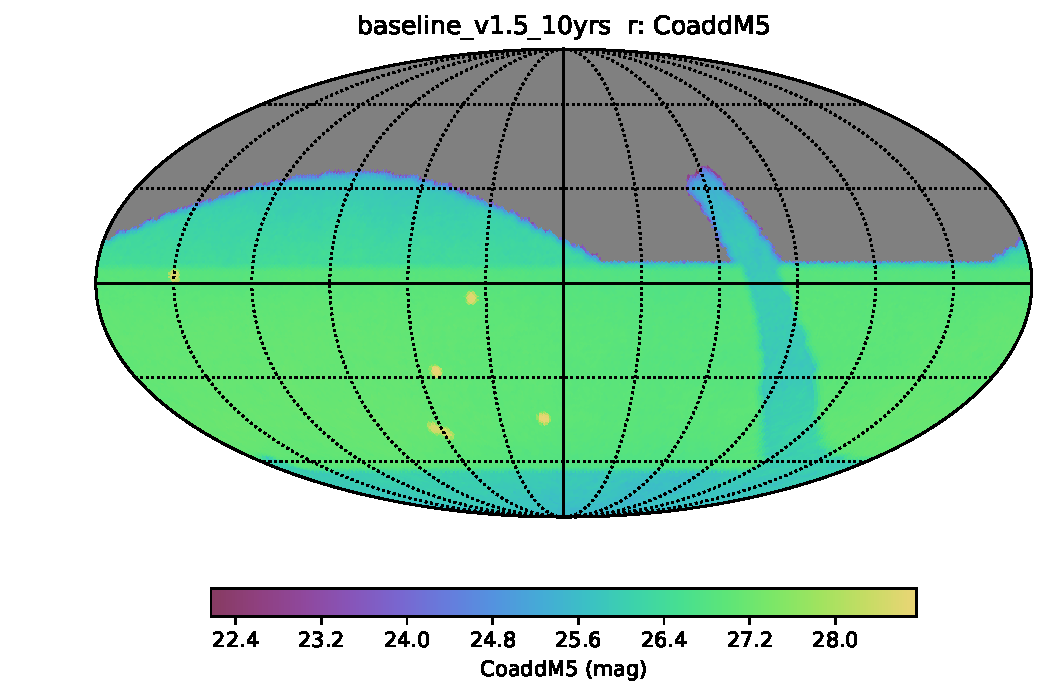
\includegraphics[width=0.5\textwidth]{metric_summary/baseline_v1.5_10yrs/baseline_v1_5_10yrs_CoaddM5_r_HEAL_SkyMap.pdf}
\caption{Final coadded depth in $r$. } \label{fig:metric-depth}
\end{figure}

\subsubsection{Number of Visits}

Compute the total number of visits for each filter.

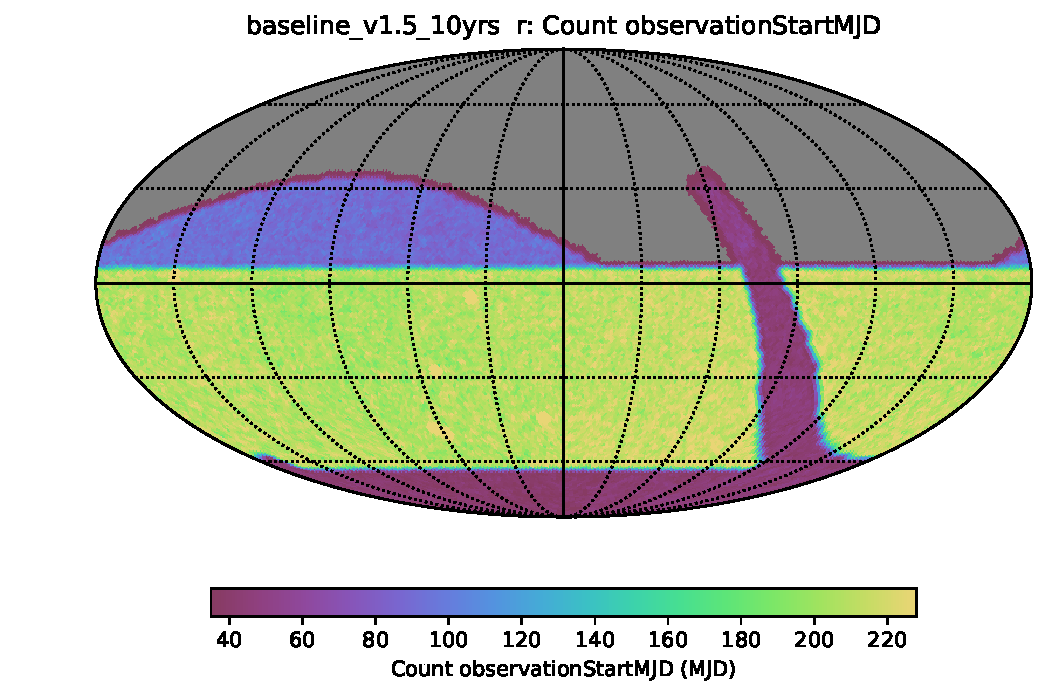
\includegraphics[width=0.5\textwidth]{metric_summary/baseline_v1.5_10yrs/baseline_v1_5_10yrs_Count_observationStartMJD_r_HEAL_SkyMap.pdf}

Also done in alt/az space (useful for checking that we are not observing at high airmass).

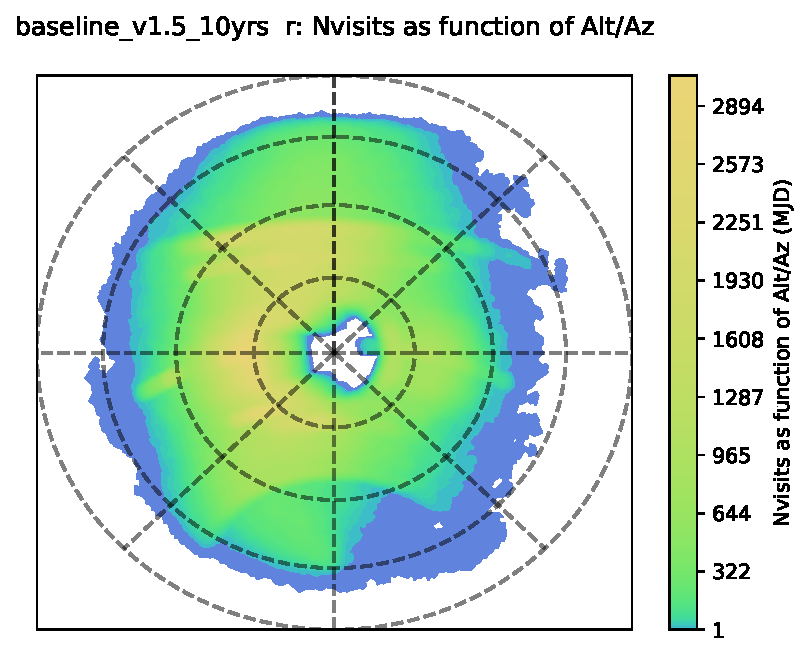
\includegraphics[width=0.5\textwidth]{metric_summary/baseline_v1.5_10yrs/baseline_v1_5_10yrs_Nvisits_as_function_of_Alt_Az_r_HEAL_SkyMap.pdf}

We have stats tables by fraction and total number for the different observing model

\subsubsection{Filter distribution}

Visualization of what filters are loaded. Useful to see if redder filters are begin used in bright time and twilight. Rapid filter changes are usually deep drilling sequences.

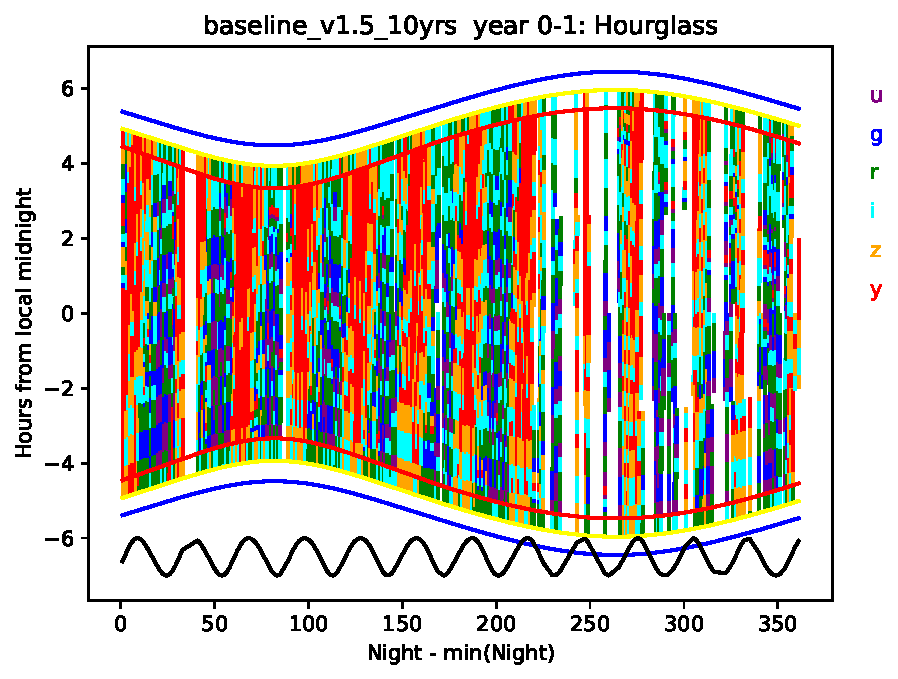
\includegraphics[width=0.5\textwidth]{metric_summary/baseline_v1.5_10yrs/baseline_v1_5_10yrs_Hourglass_year_0-1_HOUR_Hourglass.pdf}

\subsubsection{Filter Changes}

How often we change filters.

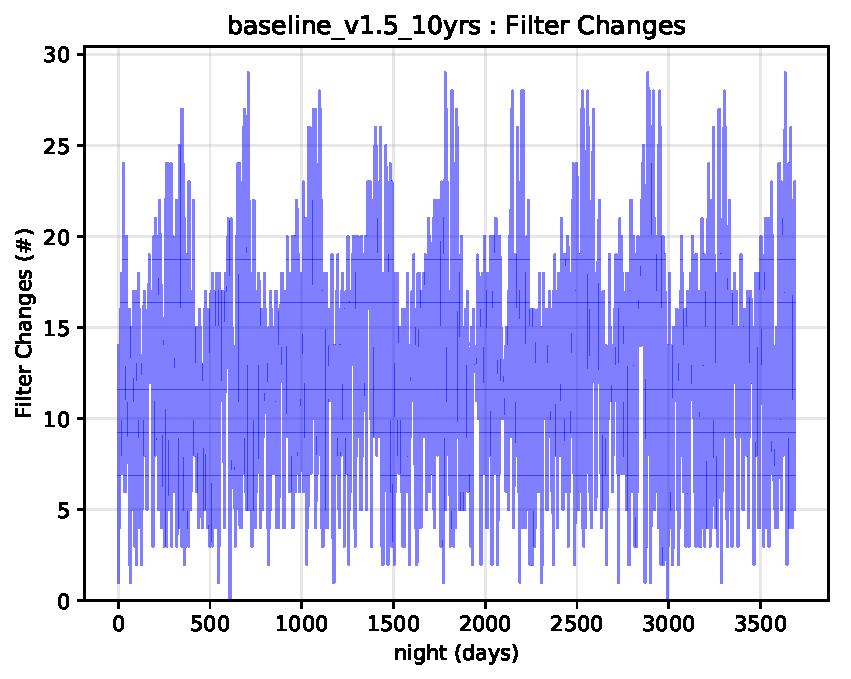
\includegraphics[width=0.5\textwidth]{metric_summary/baseline_v1.5_10yrs/baseline_v1_5_10yrs_Filter_Changes_ONED_BinnedData.pdf}

\subsubsection{Open Shutter Fraction}

How much time is the camera shutter open compared to how much time is available. Drops when there is more slewing, more filter changing, or the shutter is closed for readout between snaps.

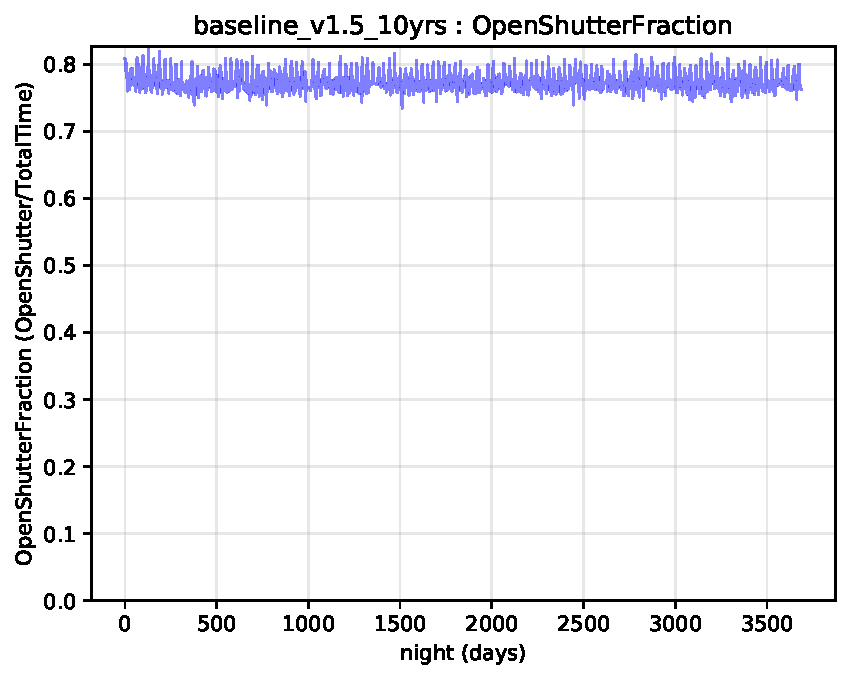
\includegraphics[width=0.5\textwidth]{metric_summary/baseline_v1.5_10yrs/baseline_v1_5_10yrs_OpenShutterFraction_ONED_BinnedData.pdf}

\subsubsection{Slew Stats}

We have plots for slew distances and times. Note the slewtime distribution has a bump around 40 seconds. Those are slews with a large enough altitude change that there is a 40s optics loop run. The peak at 120s are filter changes (filter change time is included in slewtime). Finally the peak at 160s is a filer change combined with an optics loop. Note the log scale, the vast majority of slews are under 5 seconds.

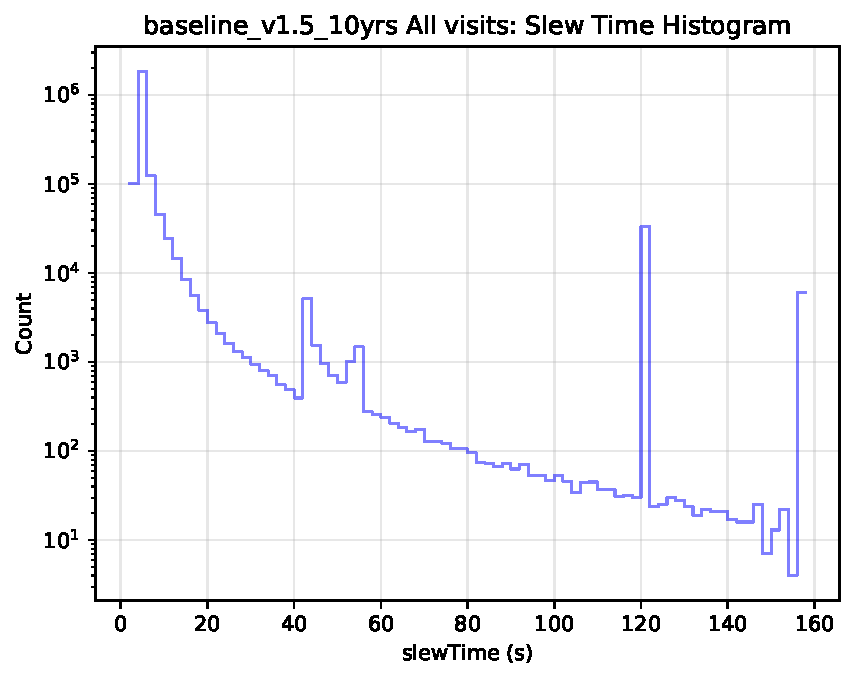
\includegraphics[width=0.5\textwidth]{metric_summary/baseline_v1.5_10yrs/baseline_v1_5_10yrs_Slew_Time_Histogram_All_visits_ONED_BinnedData.pdf}

\subsubsection{Pair Fraction}

The fraction of observations taken as pairs (e.g., can be used to identify moving objects)

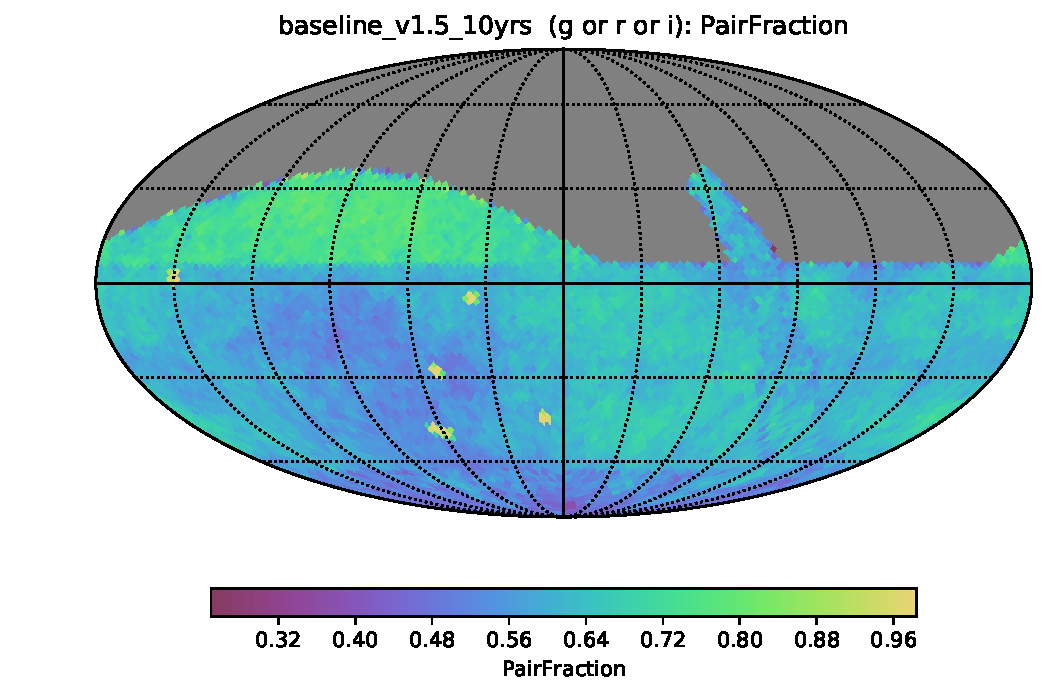
\includegraphics[width=0.5\textwidth]{metric_summary/baseline_v1.5_10yrs/baseline_v1_5_10yrs_PairFraction_g_or_r_or_i_HEAL_SkyMap.pdf}

\subsection{SRD Metrics}

\subsubsection{fO}

How well do we meet the SRD requirement to observe 18,000 square degrees 825 times.

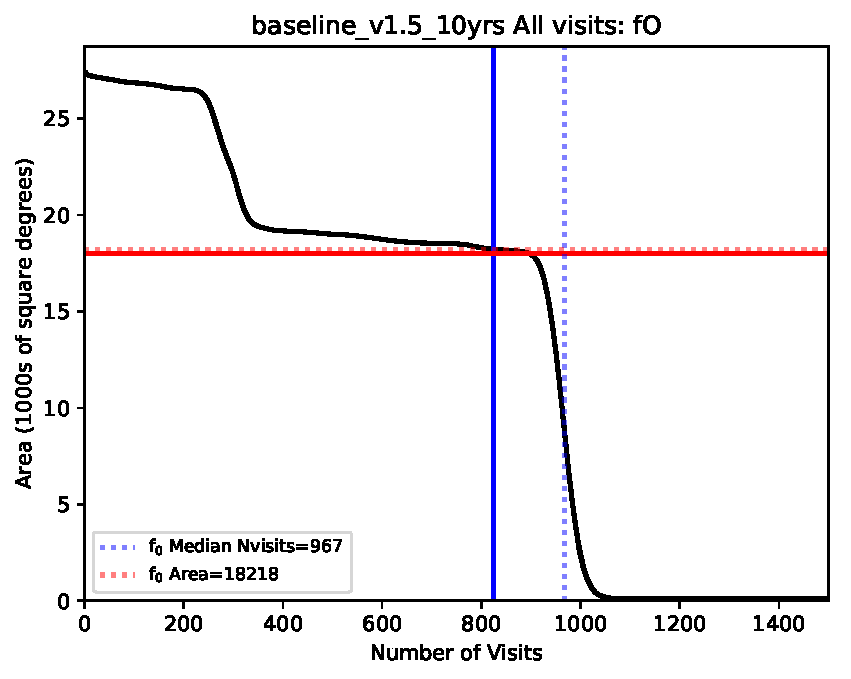
\includegraphics[width=0.5\textwidth]{metric_summary/baseline_v1.5_10yrs/baseline_v1_5_10yrs_fO_All_visits_HEAL_FO.pdf}


\subsubsection{Parallax and Proper Motion}

Estimates of how precisely we can measure proper motion and parallax for an isolated point source.

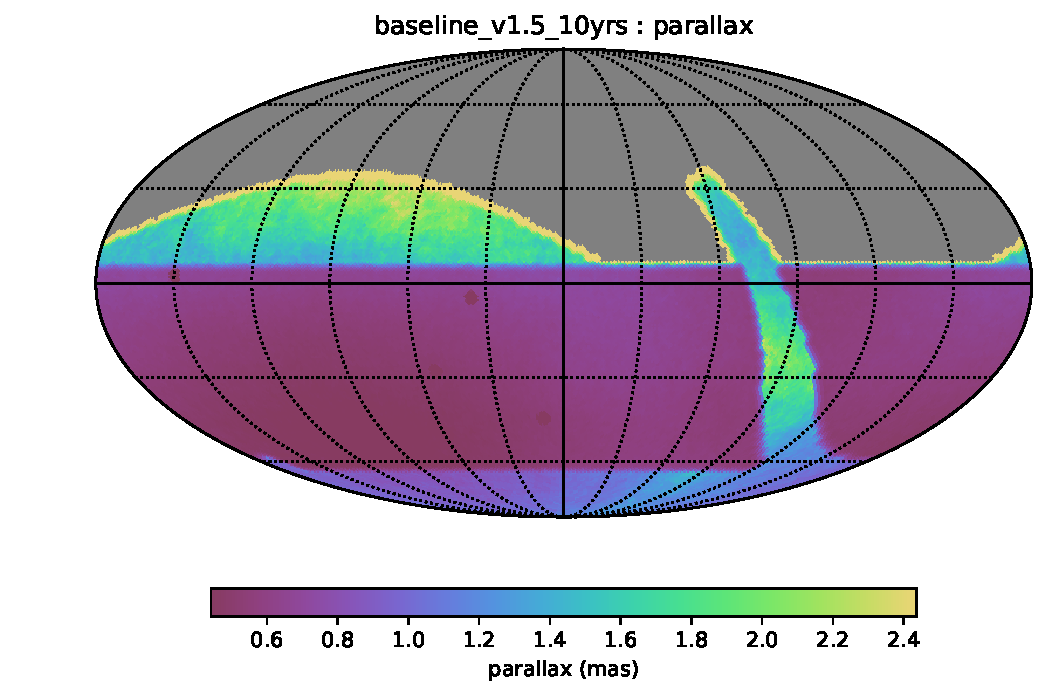
\includegraphics[width=0.5\textwidth]{metric_summary/baseline_v1.5_10yrs/baseline_v1_5_10yrs_parallax_HEAL_SkyMap.pdf}
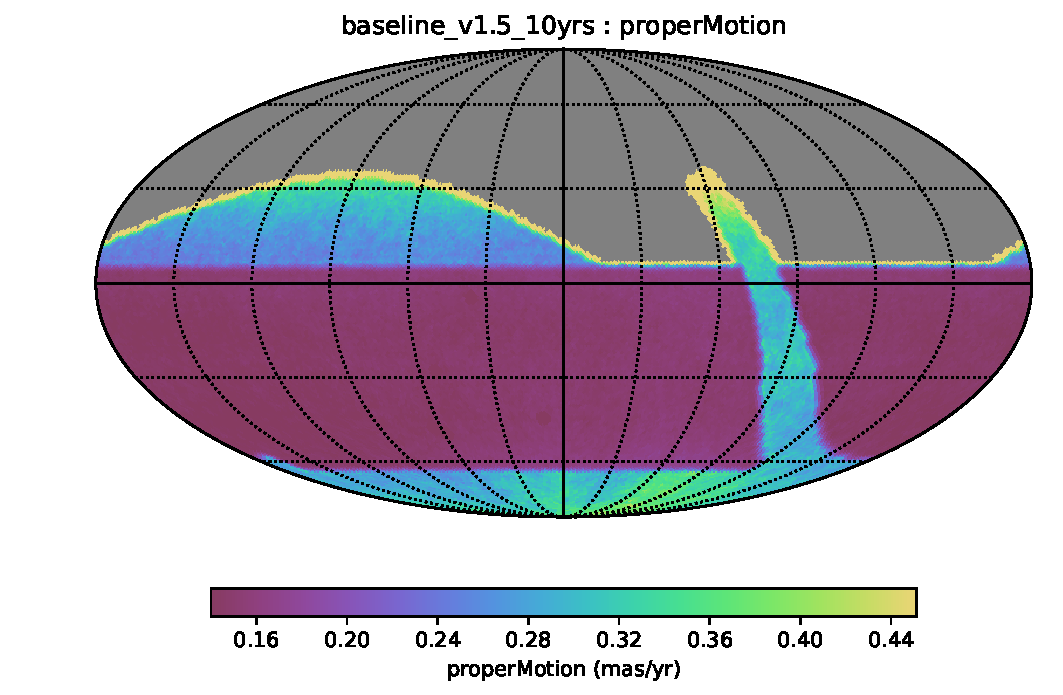
\includegraphics[width=0.5\textwidth]{metric_summary/baseline_v1.5_10yrs/baseline_v1_5_10yrs_properMotion_HEAL_SkyMap.pdf}

\subsection{Science Metrics}

\subsubsection{Supernovae}

Given a population of Type Ia SNe, we randomly distribute them on the sky and check what fraction are detected at all, how many observation of SNe there are, what fraction are detected pre-peak, and what fraction are "well sampled"

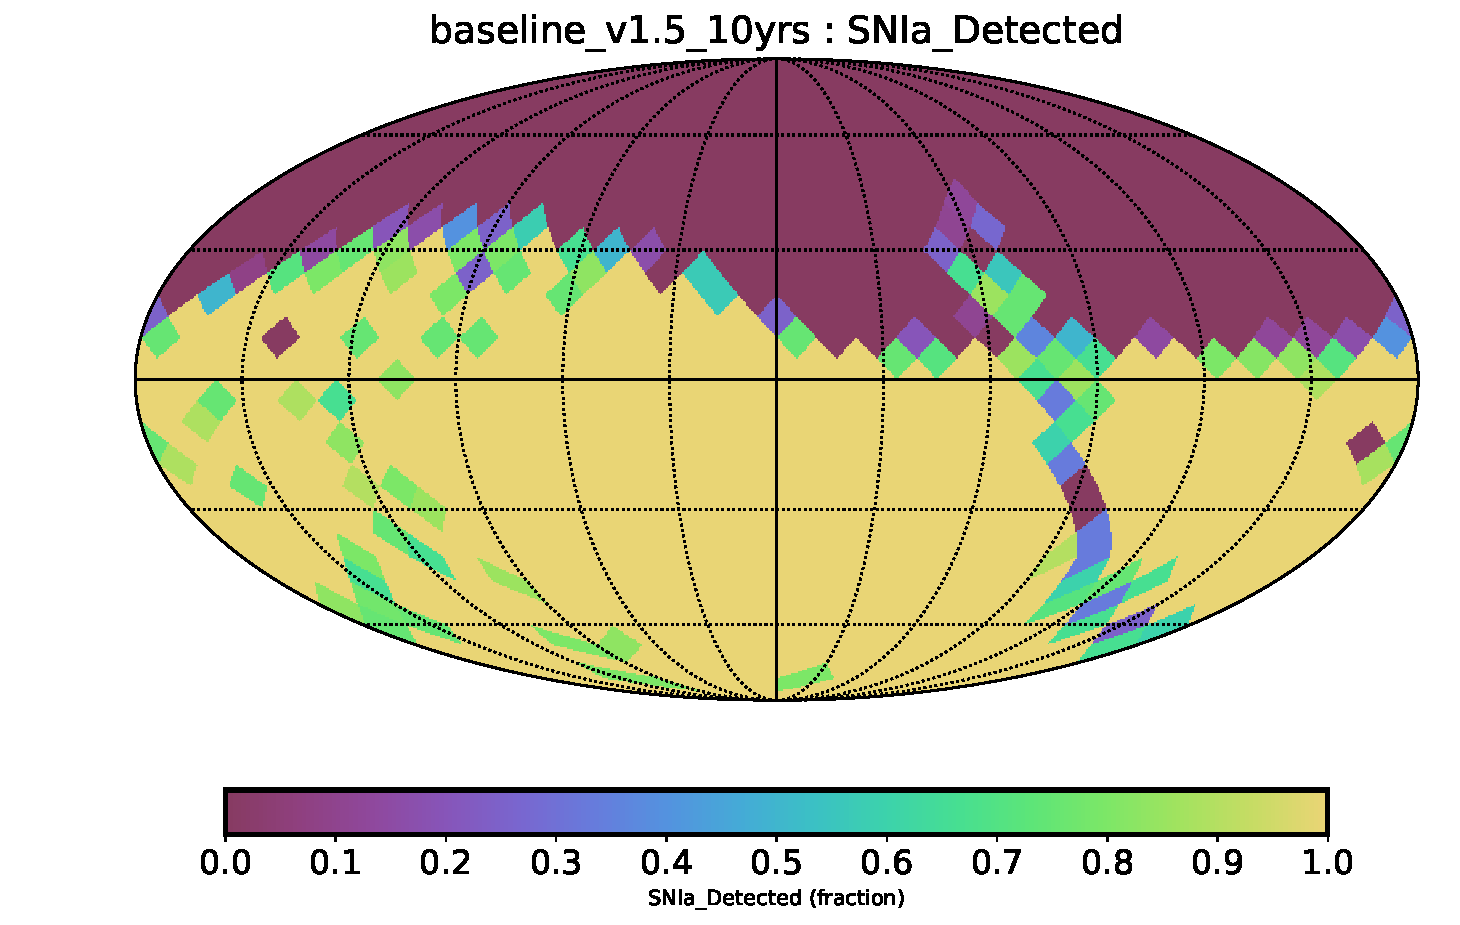
\includegraphics[width=0.5\textwidth]{metric_summary/sci_baseline_v1.5_10yrs/baseline_v1_5_10yrs_SNIa_Detected_USER_SkyMap.pdf}
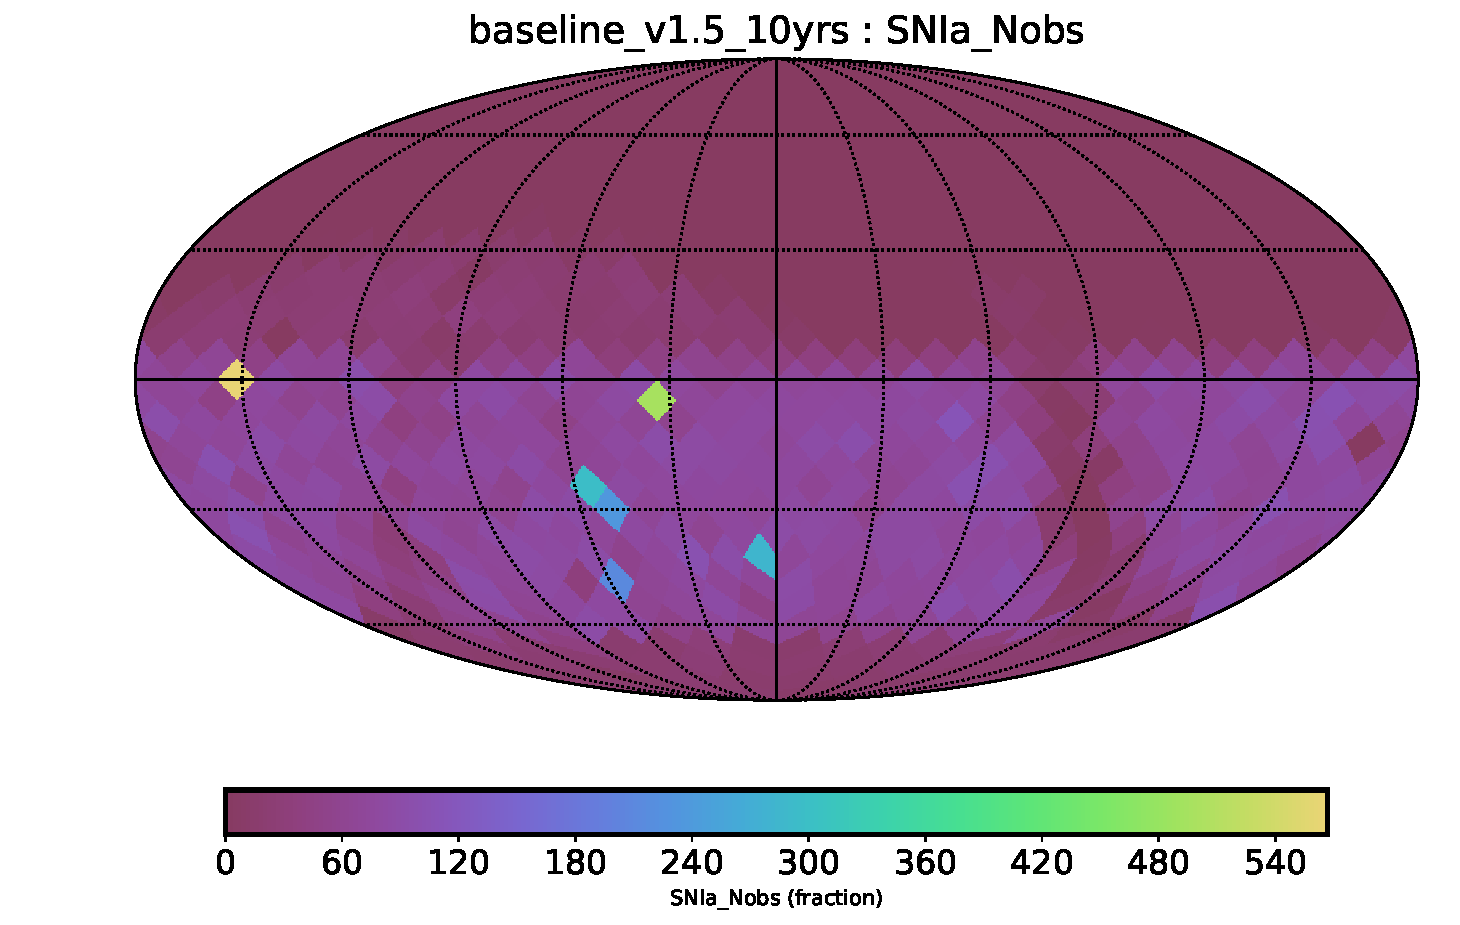
\includegraphics[width=0.5\textwidth]{metric_summary/sci_baseline_v1.5_10yrs/baseline_v1_5_10yrs_SNIa_Nobs_USER_SkyMap.pdf}
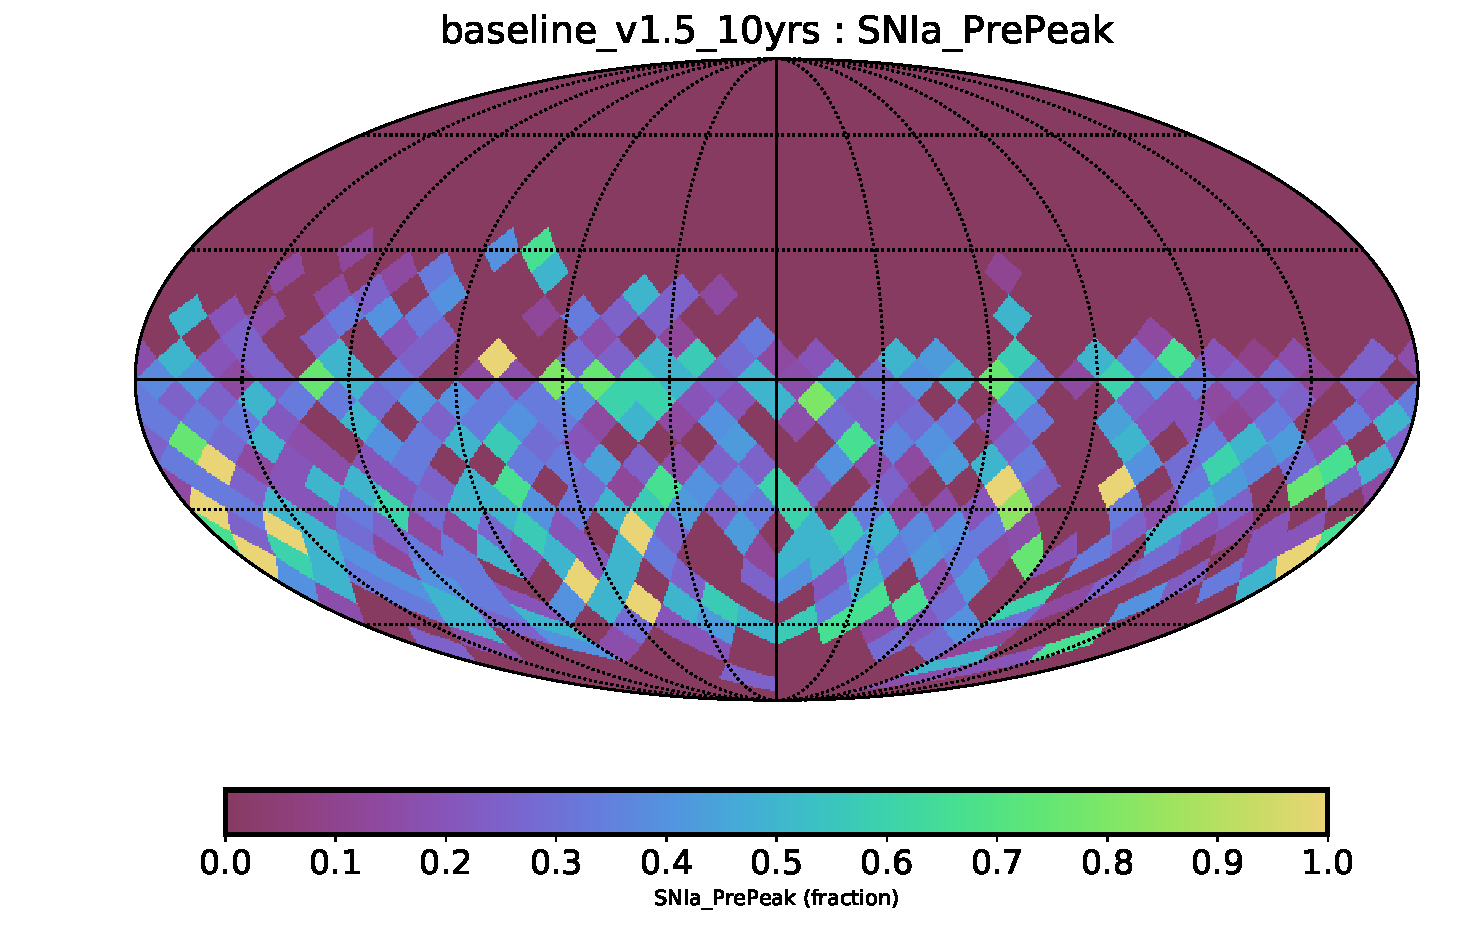
\includegraphics[width=0.5\textwidth]{metric_summary/sci_baseline_v1.5_10yrs/baseline_v1_5_10yrs_SNIa_PrePeak_USER_SkyMap.pdf}
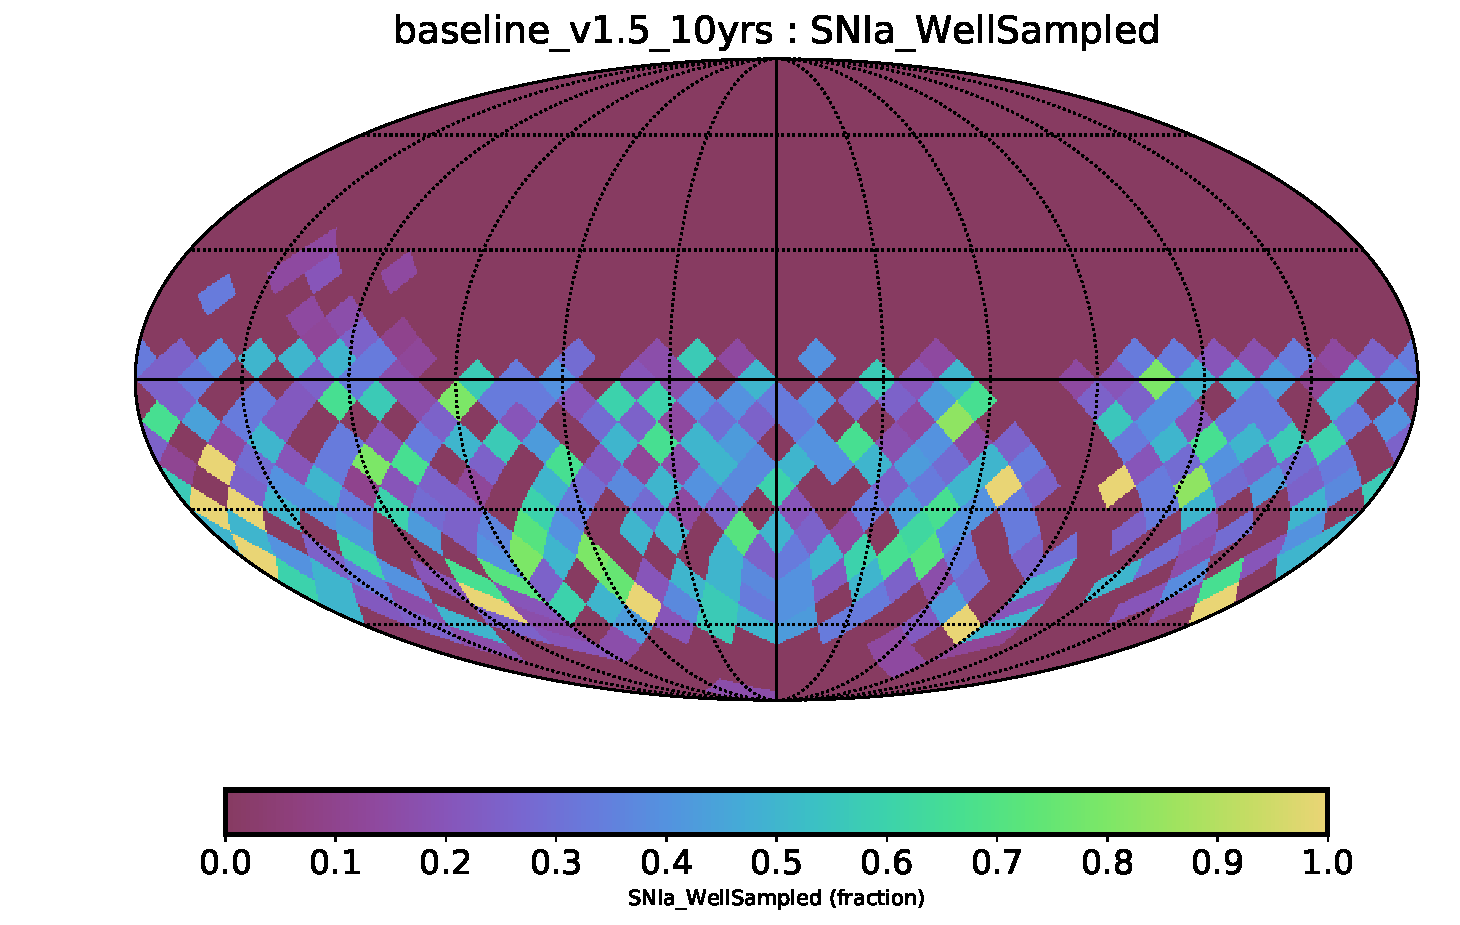
\includegraphics[width=0.5\textwidth]{metric_summary/sci_baseline_v1.5_10yrs/baseline_v1_5_10yrs_SNIa_WellSampled_USER_SkyMap.pdf}

\subsubsection{TDE}

The fraction of tidal disruption events that are recovered.
XXX--to update
%\includegraphics[width=0.5\textwidth]{metric_summary/sci_baseline_v1.5_10yrs/baseline_v1_5_10yrs_TDEsAsciiMetric_note_not_like_\%DD\%_HEAL_SkyMap.pdf}

\subsubsection{Periodic Stars}

Testing different period, amplitude, and magnitude combinations to see which periodic stars are identified.

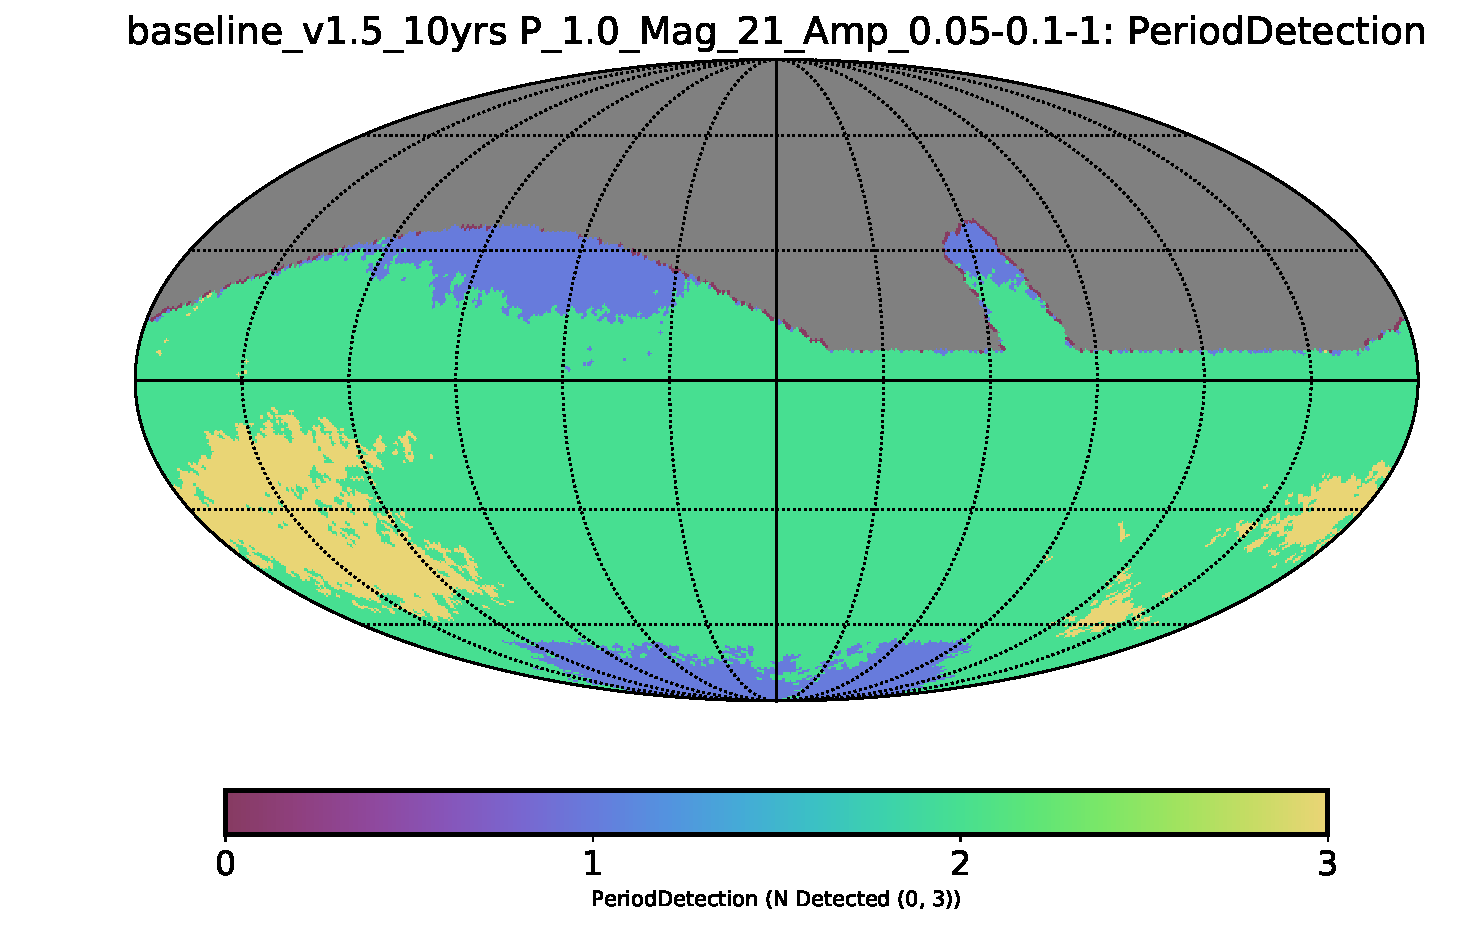
\includegraphics[width=0.5\textwidth]{metric_summary/sci_baseline_v1.5_10yrs/baseline_v1_5_10yrs_PeriodDetection_P_1_0_Mag_21_Amp_0_05-0_1-1_HEAL_SkyMap.pdf}

\subsubsection{Galaxy Counts}

The number of galaxies that can be detected (in i-band) accounting for dust extinction

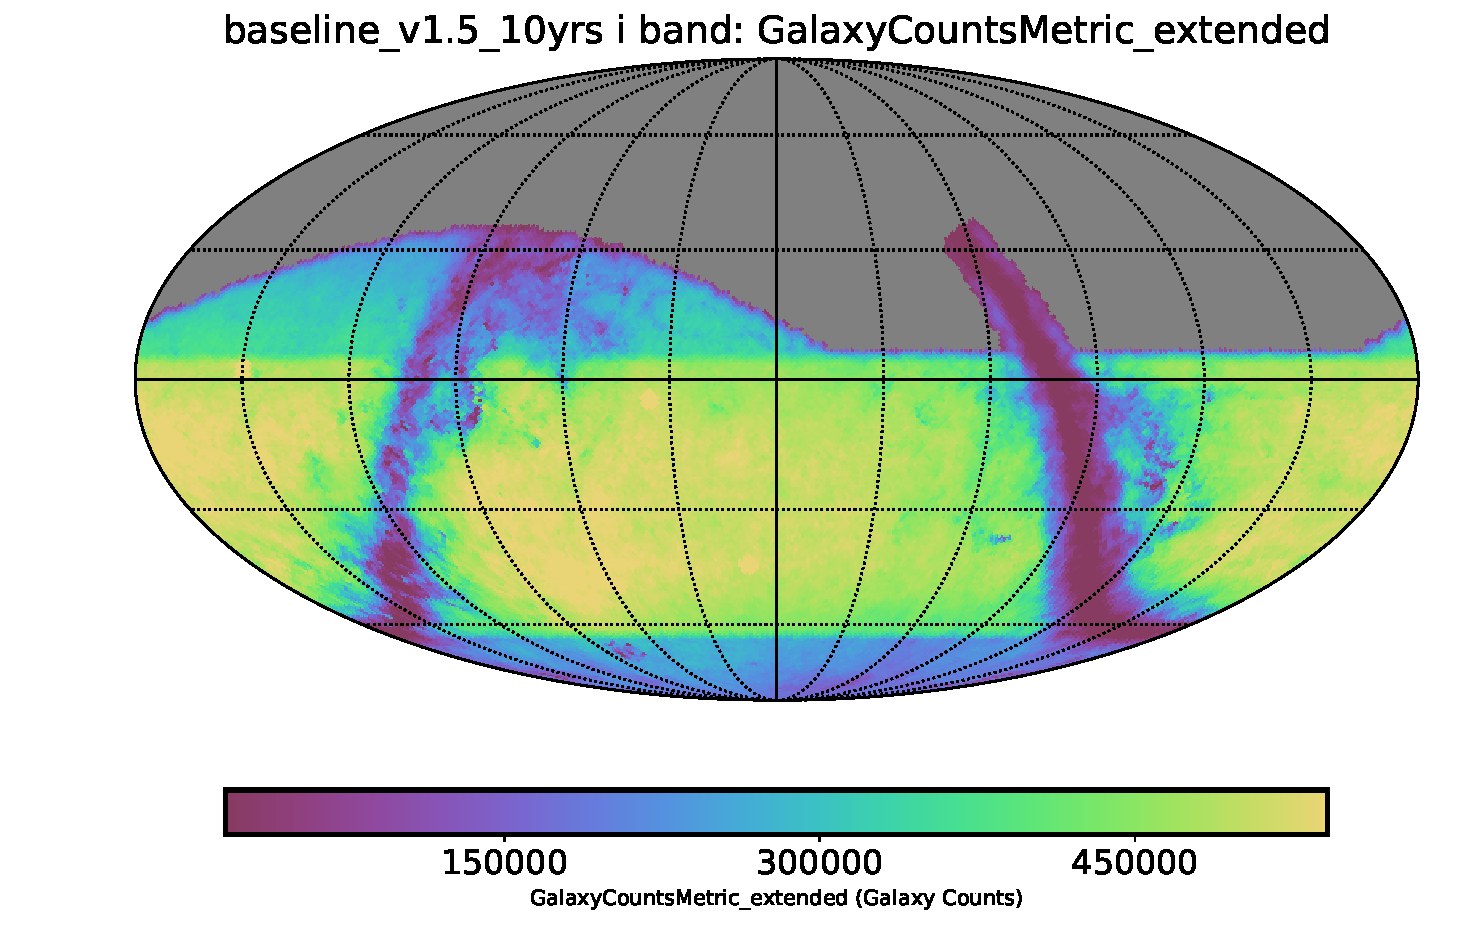
\includegraphics[width=0.5\textwidth]{metric_summary/sci_baseline_v1.5_10yrs/baseline_v1_5_10yrs_GalaxyCountsMetric_extended_i_band_HEAL_SkyMap.pdf}

\subsubsection{DDF SNe}

As with the full sky SNe recovery, only now focused on each DDF

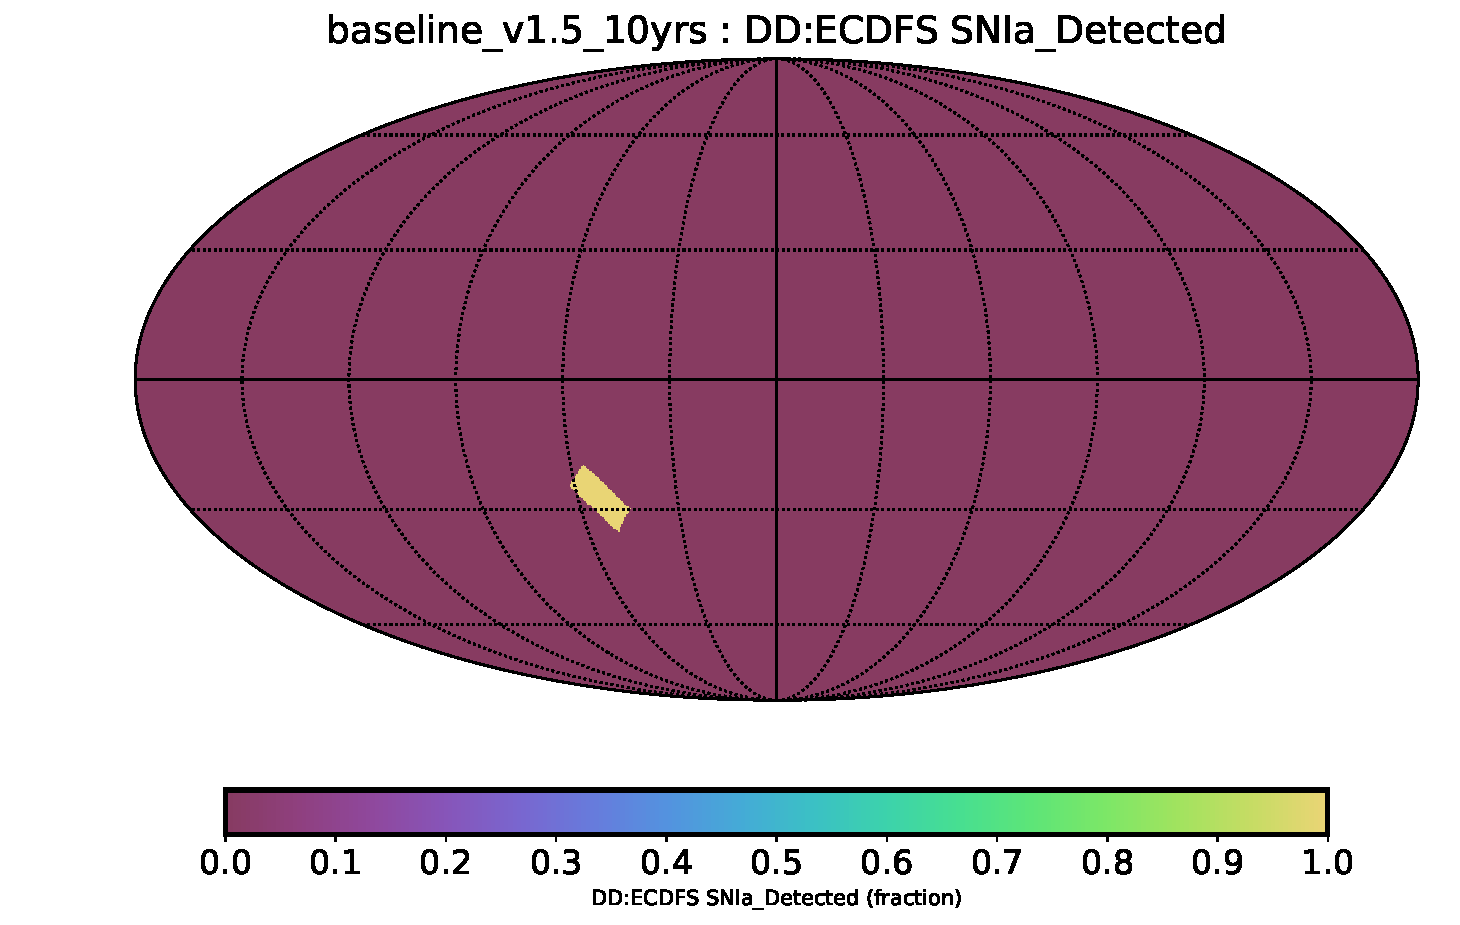
\includegraphics[width=0.5\textwidth]{metric_summary/sci_baseline_v1.5_10yrs/baseline_v1_5_10yrs_DD_ECDFS_SNIa_Detected_USER_SkyMap.pdf}

\subsubsection{DDF depth}

We compute the median depth of each DDF in each filter


\subsubsection{Annual coverage}

We check how many unique years a spot on the sky is observed per filter. Useful for determining if we will always have image subtraction templates.

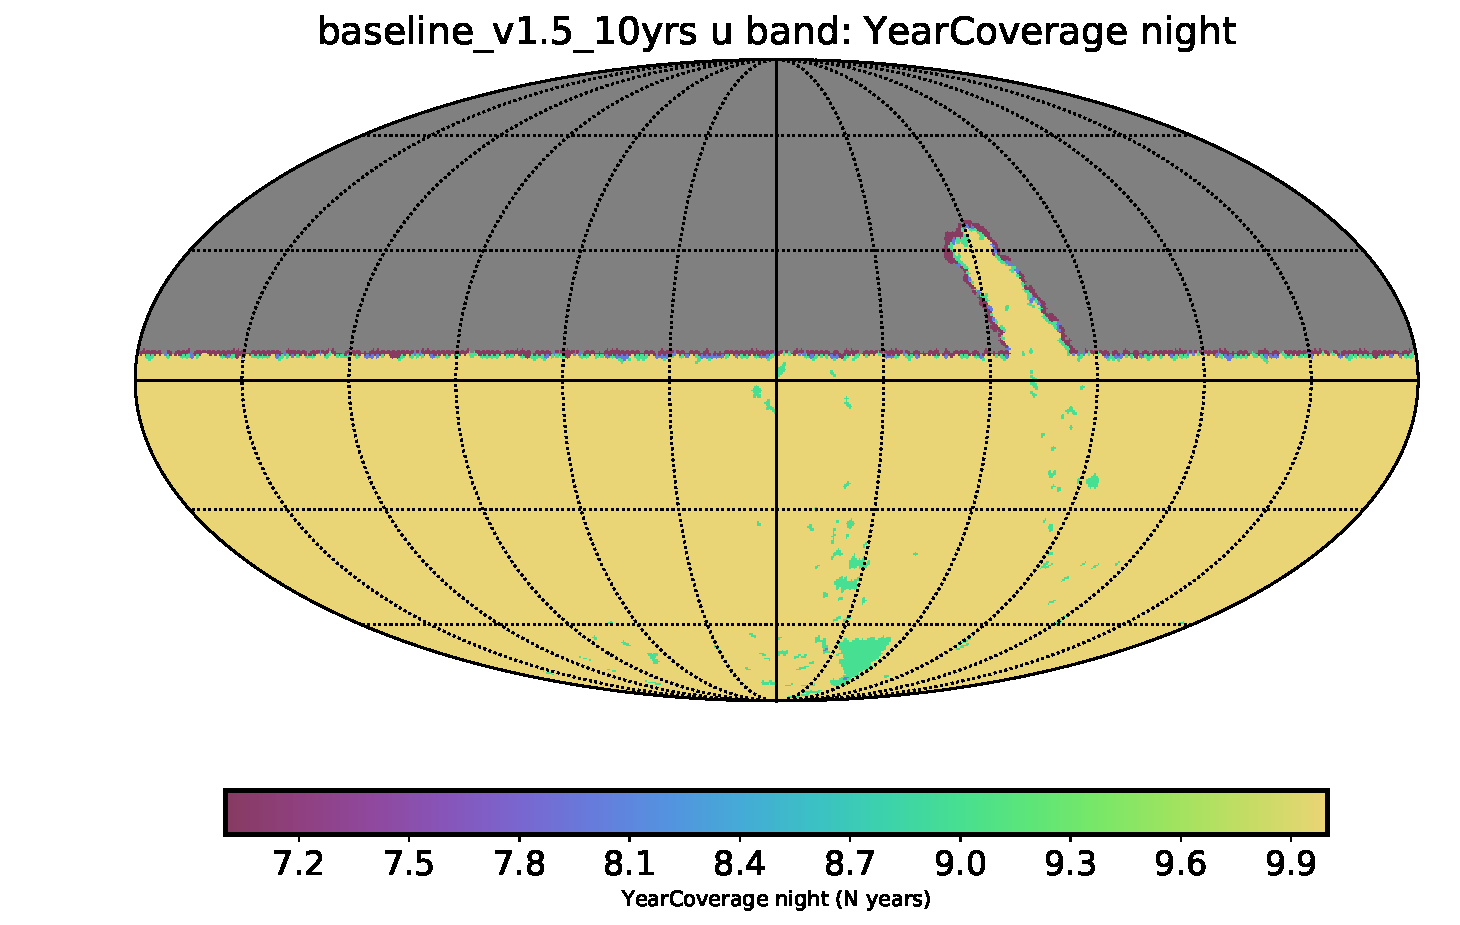
\includegraphics[width=0.5\textwidth]{metric_summary/sci_baseline_v1.5_10yrs/baseline_v1_5_10yrs_YearCoverage_night_u_band_HEAL_SkyMap.pdf}

\subsubsection{Parallax and Proper Motion}

A variety of parallax and proper motion metrics computed for point sources at r=22.5 and r=24 mag. We also check for degeneracy with DCR.

\subsubsection{Rapid Revisit}

An SRD requirement, checking how much of the sky receives at least 82 visits between 0.667 and 30.0 minutes, with at least 28 of those visits falling between 0.667 and 20.0 minutes

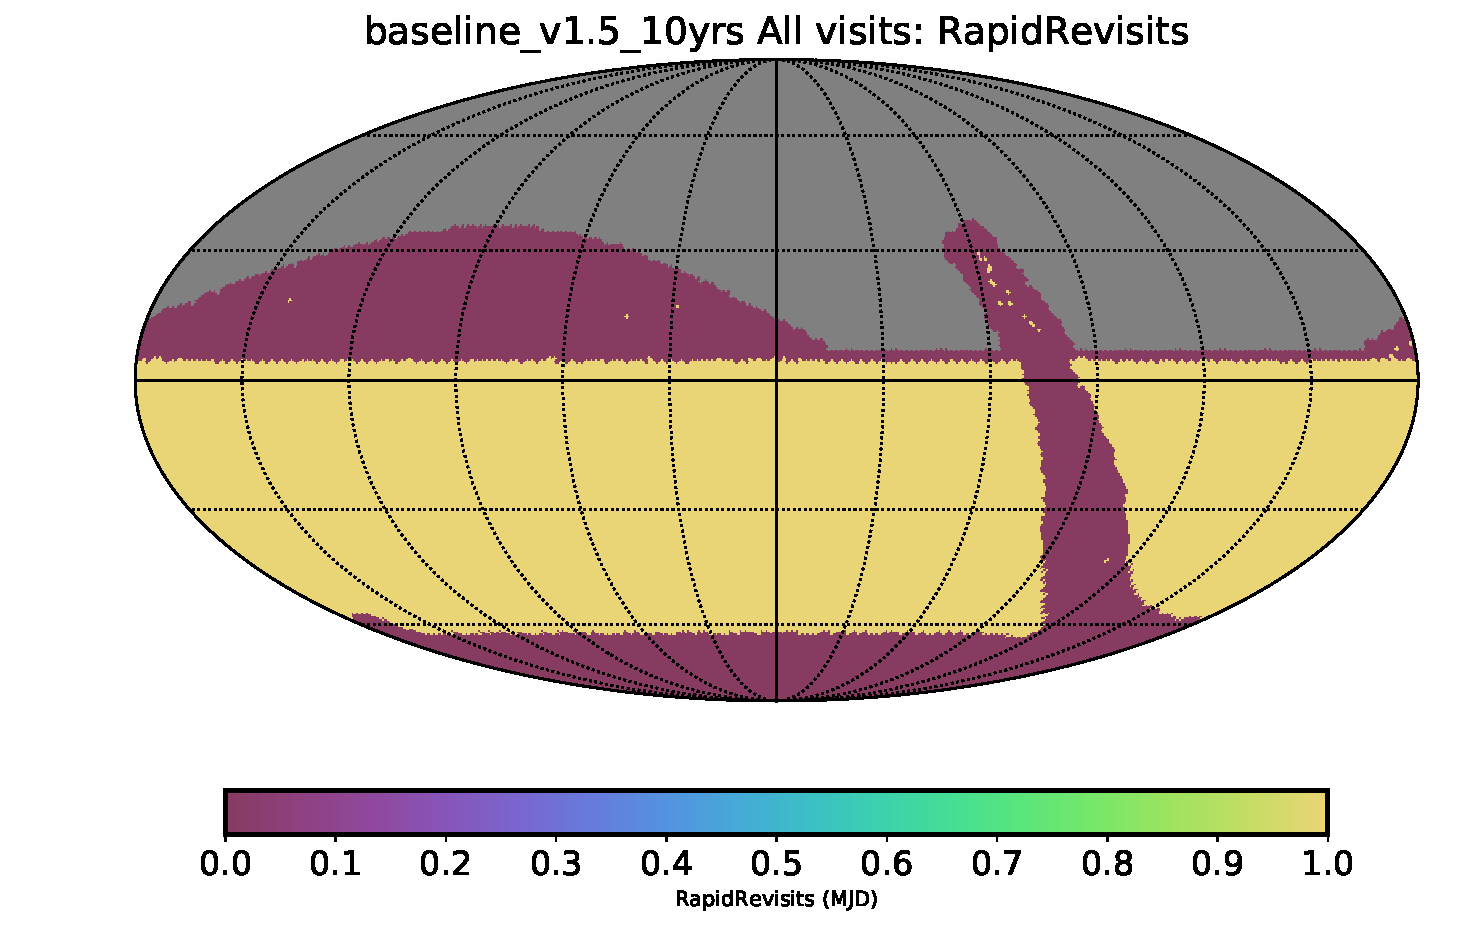
\includegraphics[width=0.5\textwidth]{metric_summary/sci_baseline_v1.5_10yrs/baseline_v1_5_10yrs_RapidRevisits_All_visits_HEAL_SkyMap.pdf}

\subsubsection{Kilonova}

Similar to the SNe metric, only now with a kilonova light curve.

\subsubsection{Camera Rotator Angle Distribution}

We look at how uniform the camera angle distribution is in each filter. For a perfectly uniform distribution between 0-360 degrees, the metric will return values of zero. For totally non-uniform (all observations taken at the same angle), the metric is one.  Because the camera rotation relative to the telescope is limited to +/- 90 degrees, the rotTelPos metric has a minimum of \~0.5. 

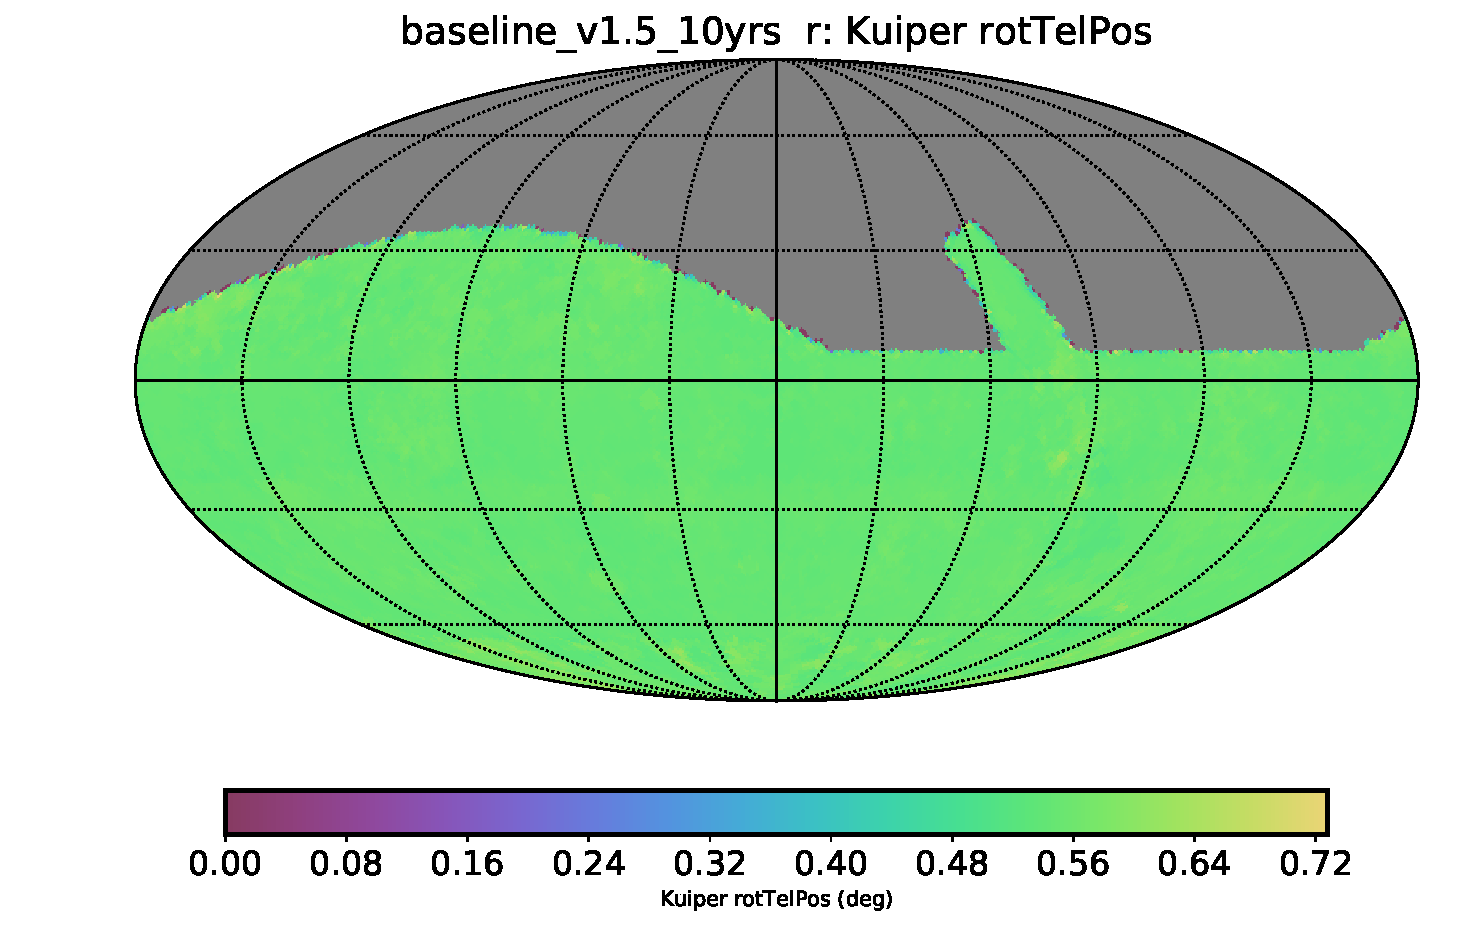
\includegraphics[width=0.5\textwidth]{metric_summary/sci_baseline_v1.5_10yrs/baseline_v1_5_10yrs_Kuiper_rotTelPos_r_HEAL_SkyMap.pdf}
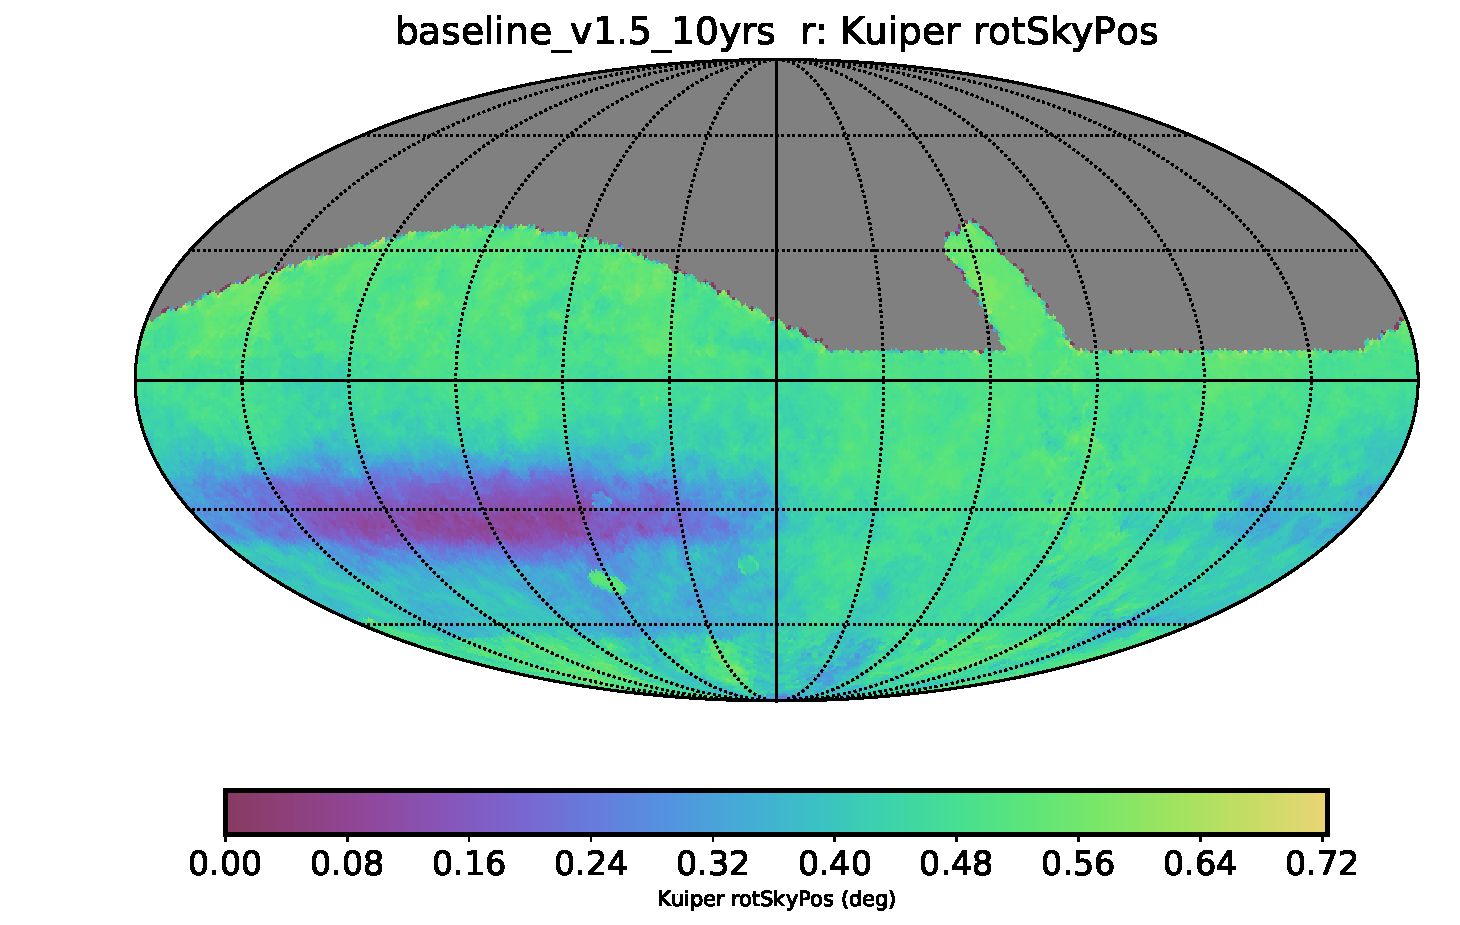
\includegraphics[width=0.5\textwidth]{metric_summary/sci_baseline_v1.5_10yrs/baseline_v1_5_10yrs_Kuiper_rotSkyPos_r_HEAL_SkyMap.pdf}


\subsubsection{Solar System Stuff}

To Do


}
